\section{W4: Stakeholder Management, Teams and Communications}

\textbf{Project Management Plan}: A formal approved document that defines how the project is executed, monitored and controlled. It may be a summary or a detailed document.

\textbf{PMP vs Project Charter}: Project charter is a summary project proposal to secure approval for the project goals and terms (useful as part of Business Case). Its primary use is to summarise key information to gain buy-ins and obtain approvals. PMP is a detailed document used to establish and manage the project.

\textbf{Stakeholder Analysis}: stakeholder identification, understanding stakeholder interests, assessing stakeholder influence, prioritising stakeholder engagement, managing stakeholder relationships.

\textbf{Stakeholder Engagement and Planning (Levels of Stakeholder Engagement)}: Unaware, Resistant, Neutral, Supportive, Champion.

\textbf{Power-Interest Grid.}

    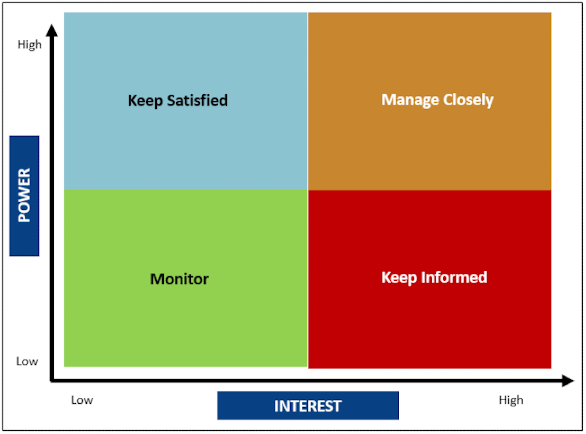
\includegraphics[width=\linewidth]{figs/SCR-20240606-jlgn.png}

\textbf{Teams and Groups}: A team is a group of people who work together to achieve a common goal. A group is a collection of individuals who interact with each other. Big difference. 

\textbf{Conway's law}: Any organization that designs a system (defined broadly) will produce a design whose structure is a copy of the organization's communication structure.

\textbf{Types of Teams}: Autocracy (one person makes decisions), Anarchy (no boss), Democracy (everyone votes).
